% Options for packages loaded elsewhere
% Options for packages loaded elsewhere
\PassOptionsToPackage{unicode}{hyperref}
\PassOptionsToPackage{hyphens}{url}
\PassOptionsToPackage{dvipsnames,svgnames,x11names}{xcolor}
%
\documentclass[
  letterpaper,
  DIV=11,
  numbers=noendperiod]{scrreprt}
\usepackage{xcolor}
\usepackage{amsmath,amssymb}
\setcounter{secnumdepth}{-\maxdimen} % remove section numbering
\usepackage{iftex}
\ifPDFTeX
  \usepackage[T1]{fontenc}
  \usepackage[utf8]{inputenc}
  \usepackage{textcomp} % provide euro and other symbols
\else % if luatex or xetex
  \usepackage{unicode-math} % this also loads fontspec
  \defaultfontfeatures{Scale=MatchLowercase}
  \defaultfontfeatures[\rmfamily]{Ligatures=TeX,Scale=1}
\fi
\usepackage{lmodern}
\ifPDFTeX\else
  % xetex/luatex font selection
\fi
% Use upquote if available, for straight quotes in verbatim environments
\IfFileExists{upquote.sty}{\usepackage{upquote}}{}
\IfFileExists{microtype.sty}{% use microtype if available
  \usepackage[]{microtype}
  \UseMicrotypeSet[protrusion]{basicmath} % disable protrusion for tt fonts
}{}
\makeatletter
\@ifundefined{KOMAClassName}{% if non-KOMA class
  \IfFileExists{parskip.sty}{%
    \usepackage{parskip}
  }{% else
    \setlength{\parindent}{0pt}
    \setlength{\parskip}{6pt plus 2pt minus 1pt}}
}{% if KOMA class
  \KOMAoptions{parskip=half}}
\makeatother
% Make \paragraph and \subparagraph free-standing
\makeatletter
\ifx\paragraph\undefined\else
  \let\oldparagraph\paragraph
  \renewcommand{\paragraph}{
    \@ifstar
      \xxxParagraphStar
      \xxxParagraphNoStar
  }
  \newcommand{\xxxParagraphStar}[1]{\oldparagraph*{#1}\mbox{}}
  \newcommand{\xxxParagraphNoStar}[1]{\oldparagraph{#1}\mbox{}}
\fi
\ifx\subparagraph\undefined\else
  \let\oldsubparagraph\subparagraph
  \renewcommand{\subparagraph}{
    \@ifstar
      \xxxSubParagraphStar
      \xxxSubParagraphNoStar
  }
  \newcommand{\xxxSubParagraphStar}[1]{\oldsubparagraph*{#1}\mbox{}}
  \newcommand{\xxxSubParagraphNoStar}[1]{\oldsubparagraph{#1}\mbox{}}
\fi
\makeatother


\usepackage{longtable,booktabs,array}
\usepackage{calc} % for calculating minipage widths
% Correct order of tables after \paragraph or \subparagraph
\usepackage{etoolbox}
\makeatletter
\patchcmd\longtable{\par}{\if@noskipsec\mbox{}\fi\par}{}{}
\makeatother
% Allow footnotes in longtable head/foot
\IfFileExists{footnotehyper.sty}{\usepackage{footnotehyper}}{\usepackage{footnote}}
\makesavenoteenv{longtable}
\usepackage{graphicx}
\makeatletter
\newsavebox\pandoc@box
\newcommand*\pandocbounded[1]{% scales image to fit in text height/width
  \sbox\pandoc@box{#1}%
  \Gscale@div\@tempa{\textheight}{\dimexpr\ht\pandoc@box+\dp\pandoc@box\relax}%
  \Gscale@div\@tempb{\linewidth}{\wd\pandoc@box}%
  \ifdim\@tempb\p@<\@tempa\p@\let\@tempa\@tempb\fi% select the smaller of both
  \ifdim\@tempa\p@<\p@\scalebox{\@tempa}{\usebox\pandoc@box}%
  \else\usebox{\pandoc@box}%
  \fi%
}
% Set default figure placement to htbp
\def\fps@figure{htbp}
\makeatother





\setlength{\emergencystretch}{3em} % prevent overfull lines

\providecommand{\tightlist}{%
  \setlength{\itemsep}{0pt}\setlength{\parskip}{0pt}}



 


\KOMAoption{captions}{tableheading}
\makeatletter
\@ifpackageloaded{caption}{}{\usepackage{caption}}
\AtBeginDocument{%
\ifdefined\contentsname
  \renewcommand*\contentsname{Table of contents}
\else
  \newcommand\contentsname{Table of contents}
\fi
\ifdefined\listfigurename
  \renewcommand*\listfigurename{List of Figures}
\else
  \newcommand\listfigurename{List of Figures}
\fi
\ifdefined\listtablename
  \renewcommand*\listtablename{List of Tables}
\else
  \newcommand\listtablename{List of Tables}
\fi
\ifdefined\figurename
  \renewcommand*\figurename{Figure}
\else
  \newcommand\figurename{Figure}
\fi
\ifdefined\tablename
  \renewcommand*\tablename{Table}
\else
  \newcommand\tablename{Table}
\fi
}
\@ifpackageloaded{float}{}{\usepackage{float}}
\floatstyle{ruled}
\@ifundefined{c@chapter}{\newfloat{codelisting}{h}{lop}}{\newfloat{codelisting}{h}{lop}[chapter]}
\floatname{codelisting}{Listing}
\newcommand*\listoflistings{\listof{codelisting}{List of Listings}}
\makeatother
\makeatletter
\makeatother
\makeatletter
\@ifpackageloaded{caption}{}{\usepackage{caption}}
\@ifpackageloaded{subcaption}{}{\usepackage{subcaption}}
\makeatother
\usepackage{bookmark}
\IfFileExists{xurl.sty}{\usepackage{xurl}}{} % add URL line breaks if available
\urlstyle{same}
\hypersetup{
  colorlinks=true,
  linkcolor={blue},
  filecolor={Maroon},
  citecolor={Blue},
  urlcolor={Blue},
  pdfcreator={LaTeX via pandoc}}


\author{}
\date{}
\begin{document}


\chapter{\texorpdfstring{\textbf{UTS-1 All About
Me}}{UTS-1 All About Me}}\label{uts-1-all-about-me}

\begin{figure}[H]

{\centering 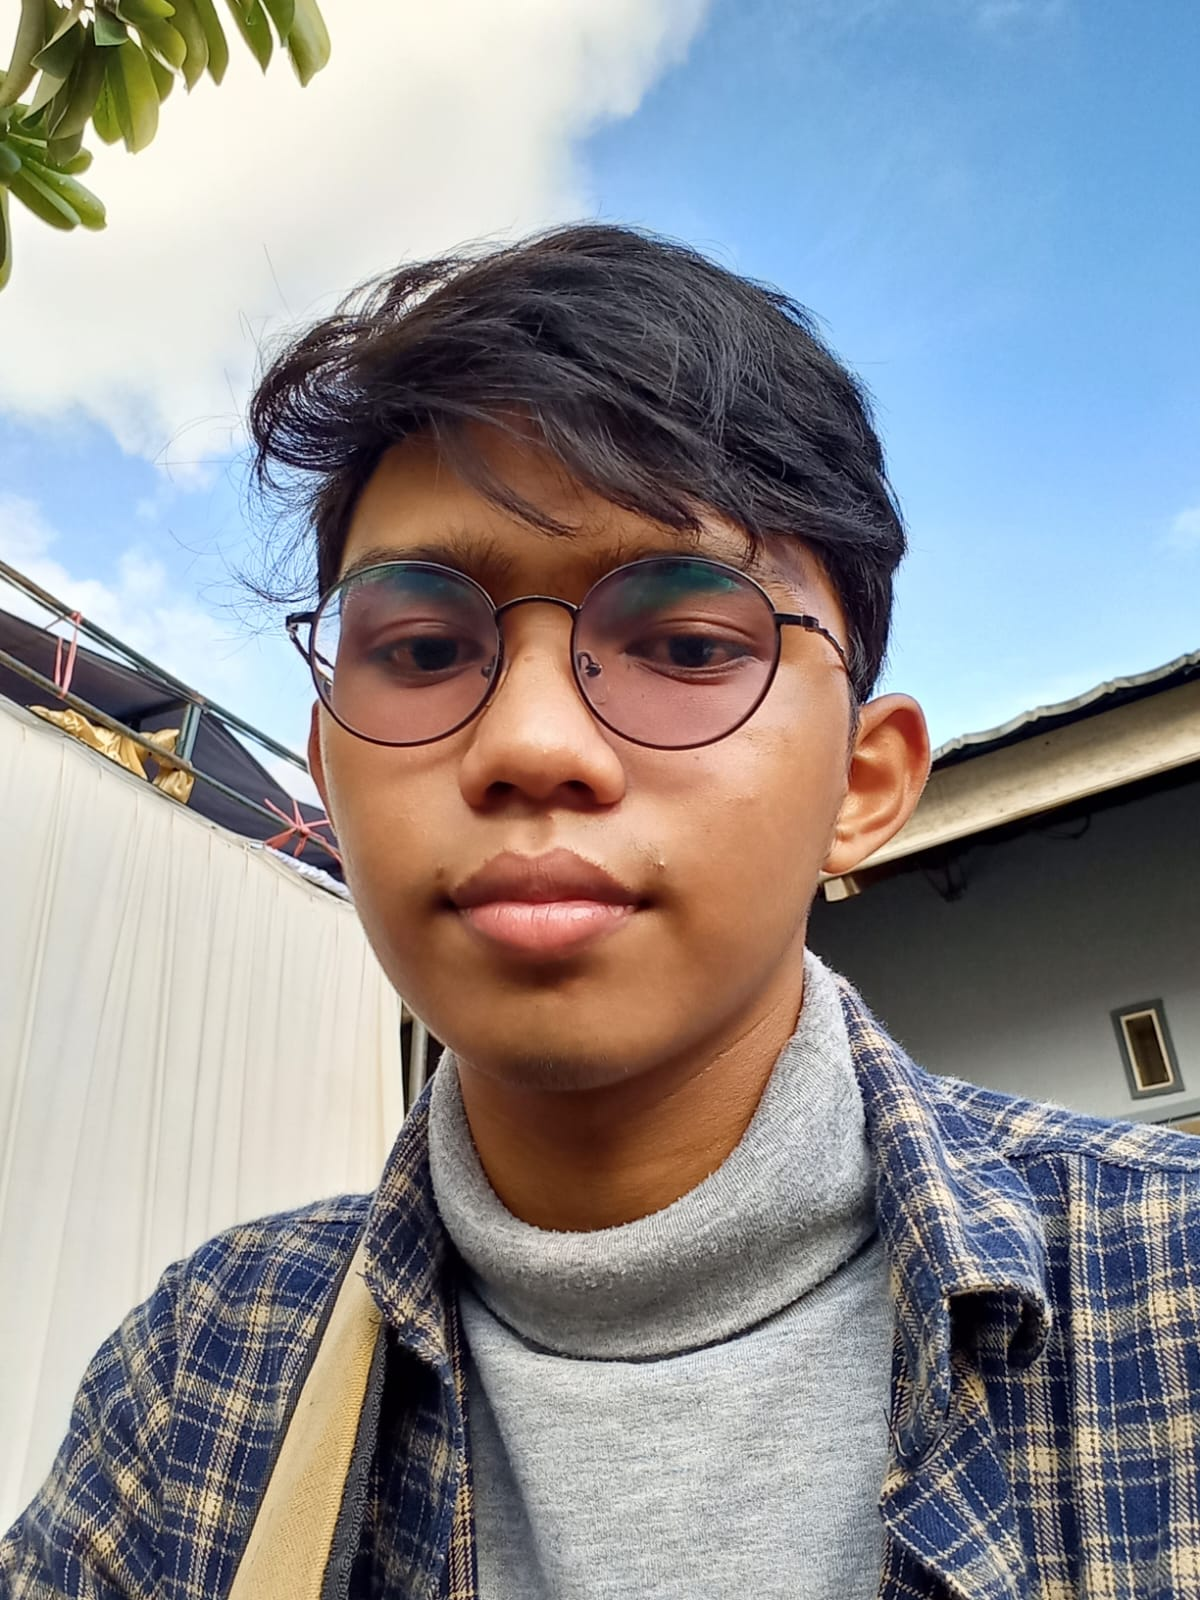
\includegraphics[width=9.5\linewidth,height=\textheight,keepaspectratio]{../images/DAFFARI.jpg}

}

\caption{About Me}

\end{figure}%

\textbf{Daffari Adiyatma} adalah mahasiswa \textbf{S1 Sistem dan
Teknologi Informasi, Institut Teknologi Bandung}, angkatan 2022.\\
Lahir di \textbf{Padang, Sumatra Barat (25 Juli 2004)} dan memiliki akar
keluarga di \textbf{Bukittinggi} dengan darah \textbf{Minang--Jawa}.\\
Ia tumbuh dalam keluarga yang menjunjung \textbf{kebebasan dalam
menentukan pilihan, pentingnya pendidikan, dan nilai kekeluargaan}.

Saat ini Daffari tinggal di Bandung untuk menempuh studi. Ia adalah
\textbf{anak pertama dari tiga bersaudara}, sosok yang dikenal logis,
analitis, dan memiliki rasa keadilan yang kuat.\\
Di luar dunia akademik, ia menikmati \textbf{membaca, menonton, bermain
musik, dan game}, yang bagi dirinya bukan sekadar hiburan, melainkan
juga sumber inspirasi moral dan refleksi diri.

LinkedIn :
\href{https://www.linkedin.com/in/daffari-adiyatma-092874255/}{daffari-adiyatma}\\
Instagram :
\href{https://www.instagram.com/dapp._25/?next=\%2F}{(\textbf{dapp.\_25?})}

\begin{center}\rule{0.5\linewidth}{0.5pt}\end{center}

\section{\texorpdfstring{\textbf{Kisah yang Membentuk Diri --- Dari
Logika, Nilai, dan Dunia
Imajinasi}}{Kisah yang Membentuk Diri --- Dari Logika, Nilai, dan Dunia Imajinasi}}\label{kisah-yang-membentuk-diri-dari-logika-nilai-dan-dunia-imajinasi}

Bagi sebagian orang, cerita hanyalah hiburan.\\
Bagi saya, cerita adalah cara untuk memahami hidup. Sejak kecil, saya
tumbuh bersama kisah-kisah dari anime, game, dan film yang menanamkan
keyakinan sederhana: bahwa \textbf{keadilan, kesetiaan, dan kebaikan}
bukan sekadar idealisme, melainkan fondasi yang menentukan apakah
seseorang layak disebut manusia seutuhnya.

Saya selalu percaya bahwa \textbf{keadilan adalah kunci kebahagiaan bagi
komunitas}. Sebab tanpa keadilan, tidak akan ada kepercayaan; dan tanpa
kepercayaan, tidak ada yang bisa dibangun bersama.\\
Namun di sisi lain, saya juga seorang \textbf{realistis}. Saya membaca
\emph{The Prince} karya Machiavelli dan justru belajar sisi positifnya:
\textbf{bahwa kekuasaan tanpa moral adalah bencana, tapi moral tanpa
realisme adalah kelemahan.}

Dalam keseharian, saya tidak menganggap dunia hitam dan putih --- lebih
sering abu-abu. Tapi dalam ruang abu-abu itulah nilai seseorang diuji:
apakah tetap teguh pada prinsip, atau hanyut dalam kepentingan sesaat.

\begin{center}\rule{0.5\linewidth}{0.5pt}\end{center}

\section{\texorpdfstring{\textbf{1. Simbolisme Identitas --- Antara
Logika, Kekuasaan, dan
Kemanusiaan}}{1. Simbolisme Identitas --- Antara Logika, Kekuasaan, dan Kemanusiaan}}\label{simbolisme-identitas-antara-logika-kekuasaan-dan-kemanusiaan}

Jika saya harus menuliskan refleksi diri dalam tokoh-tokoh simbolik,
maka saya melihat diri saya di antara \textbf{Kazuya Souma},
\textbf{King Baldwin IV}, \textbf{Salahuddin Al-Ayyubi}, dan
\textbf{Lelouch vi Britannia} --- empat pemimpin dari dunia yang
berbeda, namun diikat oleh satu benang merah: \textbf{logika yang
berakar pada nilai kemanusiaan.}

Dari \textbf{Kazuya Souma}, saya belajar bahwa rasionalitas dan empati
bukanlah dua hal yang saling bertentangan. Ia membangun kerajaannya
bukan dengan pedang, melainkan dengan kebijakan dan perhitungan. Ia
memperlihatkan bahwa menjadi pemimpin berarti \emph{mengelola sistem,
bukan memerintah manusia.}\\
Souma melambangkan ideal saya: \emph{seorang pemimpin yang bekerja
dengan akal, tapi memutuskan dengan hati.}

Dari \textbf{King Baldwin IV}, saya belajar kebijaksanaan dalam
kesunyian. Ia tahu kekuasaannya fana, tubuhnya rapuh, tapi jiwanya
teguh. Ia menolak memerintah dengan amarah, dan justru menaklukkan dunia
lewat kendali diri.\\
Baldwin mengajarkan saya bahwa \emph{keadilan tanpa kebijaksanaan akan
melahirkan kekerasan, dan kekuasaan tanpa pengendalian diri akan
melahirkan kejatuhan.}

Berhadapan dengannya dalam sejarah adalah \textbf{Salahuddin Al-Ayyubi},
simbol lain dari kebesaran hati. Ia memimpin dengan keberanian dan belas
kasih, menang tanpa kesombongan, dan menegakkan kehormatan bahkan kepada
musuhnya.\\
Salahuddin memperlihatkan bahwa \emph{iman dan kemanusiaan dapat
berjalan beriringan tanpa saling meniadakan.}

Sementara \textbf{Lelouch vi Britannia} mengingatkan saya akan kenyataan
bahwa setiap keputusan besar membawa harga yang harus dibayar. Ia
memahami bahwa dunia sering kali bergerak bukan karena kebenaran,
melainkan karena persepsi.\\
Lelouch melambangkan keberanian dalam mengambil keputusan sulit --- dan
kesadaran bahwa pengorbanan sering kali menjadi bentuk keadilan terakhir
yang tersisa.

Empat sosok ini bukanlah idola, melainkan \emph{cermin filosofis} bagi
empat pilar kepribadian yang saya pegang:

\begin{itemize}
\tightlist
\item
  \textbf{Souma} → logika dan sistematika\\
\item
  \textbf{Baldwin} → kebijaksanaan dan pengendalian diri\\
\item
  \textbf{Salahuddin} → empati dan kehormatan\\
\item
  \textbf{Lelouch} → keberanian dan tanggung jawab moral
\end{itemize}

\begin{quote}
\textbf{Keadilan memberi arah, kebijaksanaan memberi batas, empati
memberi makna, dan keberanian memberi jalan.}\\
Di antara keempatnya, saya menemukan ruang bagi diri saya sendiri ---
seorang manusia yang ingin berpikir dengan kepala yang jernih,
berperilaku dengan hati yang tulus, dan bertindak dengan tanggung jawab
yang sadar akan akibatnya.
\end{quote}

\begin{center}\rule{0.5\linewidth}{0.5pt}\end{center}

\section{\texorpdfstring{\textbf{2. Struktur Diri --- Menemukan Narasi
Personal}}{2. Struktur Diri --- Menemukan Narasi Personal}}\label{struktur-diri-menemukan-narasi-personal}

Dalam kerangka teori \emph{self-concept} dan \emph{identitas naratif}
(McAdams, 1993) sebagaimana dijelaskan pada materi \emph{Memahami
Komunikasi Diri dan Pementasan Diri}, kepribadian manusia terbentuk dari
tiga lapisan:

\begin{enumerate}
\def\labelenumi{\arabic{enumi}.}
\tightlist
\item
  \textbf{Sifat dasar (trait level)} --- cara alami saya berpikir dan
  berperilaku: logis, analitis, tenang, tetapi frontal saat
  mempertanyakan sesuatu.\\
\item
  \textbf{Kepedulian pribadi (personal concern)} --- nilai yang saya
  pegang: keadilan, kesetiaan, dan kebaikan.\\
\item
  \textbf{Identitas naratif (narrative identity)} --- kisah hidup yang
  saya bangun untuk memaknai siapa saya dan mengapa saya bertindak
  demikian.
\end{enumerate}

Ketiga lapisan ini berpadu dalam satu prinsip: \textbf{menjadi rasional
tanpa kehilangan rasa kemanusiaan.}\\
Saya berusaha menjadi seseorang yang tidak hanya berpikir dengan kepala,
tetapi juga dengan hati yang tahu kapan harus berhenti berdebat dan
mulai memahami.

\begin{center}\rule{0.5\linewidth}{0.5pt}\end{center}

\section{\texorpdfstring{\textbf{3. Refleksi --- Agensi dan Daya Tarik
Personal}}{3. Refleksi --- Agensi dan Daya Tarik Personal}}\label{refleksi-agensi-dan-daya-tarik-personal}

Dalam komunikasi interpersonal, \emph{daya tarik} tidak sekadar soal
penampilan, tetapi tentang \textbf{kemampuan menampilkan diri dengan
jujur dan konsisten}.\\
Konsep ini berkaitan dengan \emph{agensi} --- keyakinan bahwa kita
adalah aktor utama dalam kisah hidup kita sendiri.

Sebagai pribadi yang logis dan realistis, saya percaya bahwa
\emph{tindakan sadar} adalah bentuk komunikasi tertinggi.\\
Kita bisa memilih untuk adil, setia, dan berbuat baik, bahkan di tengah
dunia yang mungkin tidak selalu melakukan hal yang sama kepada kita.\\
Di situlah letak \emph{agensi diri} saya: dalam kesadaran untuk tetap
menjadi diri sendiri, bukan korban keadaan.

\begin{center}\rule{0.5\linewidth}{0.5pt}\end{center}

\section{\texorpdfstring{\textbf{4. Kesimpulan --- Rasionalitas,
Keberanian, dan
Nilai}}{4. Kesimpulan --- Rasionalitas, Keberanian, dan Nilai}}\label{kesimpulan-rasionalitas-keberanian-dan-nilai}

Saya mungkin bukan pencerita ulung, tetapi saya paham bahwa setiap
keputusan adalah bab dalam buku hidup yang saya tulis sendiri.\\
Saya memilih untuk menjalani hidup dengan logika sebagai panduan, nilai
sebagai jangkar, dan keberanian sebagai tinta yang menulis perjalanan
itu.

\begin{quote}
\textbf{Saya ingin dikenal sebagai seseorang yang berpikir dengan
kepala, bertindak dengan hati, dan berdiri di atas keadilan, bahkan
ketika sendirian.}
\end{quote}

\begin{center}\rule{0.5\linewidth}{0.5pt}\end{center}

\section{\texorpdfstring{\textbf{Refleksi Konseptual --- Komunikasi Diri
dan Daya Tarik
Pribadi}}{Refleksi Konseptual --- Komunikasi Diri dan Daya Tarik Pribadi}}\label{refleksi-konseptual-komunikasi-diri-dan-daya-tarik-pribadi}

Tulisan ini merupakan bentuk \emph{komunikasi intrapersonal} --- sebuah
dialog antara logika, nilai, dan aspirasi yang membentuk identitas
diri.\\
Dalam konteks \emph{Komunikasi Interpersonal}, saya memahami bahwa
\textbf{self-concept} bersifat dinamis: ia tumbuh, beradaptasi, dan
berinteraksi dengan lingkungan sosial.

Pementasan diri (\emph{self-presentation}) yang saya lakukan bukanlah
topeng, melainkan ekspresi autentik dari konsistensi antara keyakinan
dan tindakan.\\
Inilah inti \emph{daya tarik pribadi}: menjadi seseorang yang jelas bagi
dirinya sendiri, sehingga orang lain pun dapat melihatnya dengan jelas.

Dengan demikian, \emph{All About Me} bukan hanya pengenalan pribadi,
tetapi juga latihan reflektif untuk memahami bagaimana saya dapat
\textbf{berkomunikasi secara efektif, etis, dan autentik} dalam
kehidupan pribadi maupun profesional.




\end{document}
